\begin{definition}
Let $S$ be a closed set.
\begin{enumerate}
\item A (codimension $1$ lamination) \dfn{flow box} for $S$ is a Lipschitz chart in which $S$ can be expressed as $K \times N \subseteq \RR^d$ for some closed $K \subseteq \RR$ and open connected $N \subseteq \RR^{d - 1}$.
\item A (codimension $1$) \dfn{lamination} $\lambda$ in $M$, with support $S$, consists of an atlas of lamination flow boxes whose transition maps preserve the local product structure.
\item A \dfn{leaf} of $\lambda$ is a connected subset of $\supp \lambda = S$ which is locally modeled on the fibers $\{k\} \times N$, $k \in K$.
\item The lamination $\lambda$ is \dfn{minimal} if every leaf of $\lambda$ is $C^2$ and has zero mean curvature.
\end{enumerate}
\end{definition}

See \cite{Morgan88} for a detailed treatment of laminations.
Note carefully that the term ``minimal lamination'' is overloaded: in \cite{daskalopoulos2020transverse,casson_bleiler_1988} it refers to laminations which are minimal with respect to inclusion, which has nothing to do with the condition on leaves.
In the surface case $d = 2$, minimal laminations are also called \dfn{geodesic laminations}, though we will not use this terminology.

\begin{definition}
Let $\lambda$ be a lamination, let $\psi_{ij}$, $i,j \in I$, be the transition maps for $\lambda$, and let $(\chi_i)$ be a partition of unity subordinate to $(\psi_{ij})$.
\begin{enumerate}
\item $\lambda$ is \dfn{measured} if it is equipped with Radon measures $\mu_i$ on each set of leaves $K_i$, $i \in I$, such that $\psi_{ij}^* \mu_i = \mu_j$; in that case we say that $\mu = (\mu_i)$ is a \dfn{transverse measure} to $\lambda$.
\item $\lambda$ is \dfn{oriented} if $\psi_{ij}$ are oriented.
\item If $\lambda$ is a measured oriented lamination, then the \dfn{Ruelle-Sullivan current} $T_\lambda$ of $\lambda$ satisfies, for every $d-1$-form $\varphi$,
$$\int_M T_\lambda \wedge \varphi := \sum_{i \in I} \int_{K_i} \int_{\{k\} \times N_i} \chi_i \varphi \dif \mu_i(k).$$
\end{enumerate}
\end{definition}

Of course, the choice of partition of unity $(\chi_i)$ in the definition of Ruelle-Sullivan current is immaterial.
The Ruelle-Sullivan current is always closed, $\dif T_\lambda = 0$, so it can be locally written $T_\lambda = \dif u$.
The main theorem of this paper characterizes the functions $u$ for which $\dif u$ is a Ruelle-Sullivan current for a minimal lamination:

\begin{mainthm}\label{main thm}
Let $2 \leq d \leq 4$ and suppose that $M$ has constant sectional curvature.
\begin{enumerate}
\item Let $u$ be a function of least gradient.
Then
\begin{enumerate}
\item for every $y \in \RR$, $\partial \{u > y\}$ is either empty or an analytic embedded hypersurface,
\item $\bigcup_{y \in \RR} \partial \{u > y\}$ is the support of a minimal measured oriented lamination $\lambda$ whose leaves are the connected components of the hypersurfaces $\partial \{u > y\}$, and
\item the Ruelle-Sullivan current of $\lambda$ is $\dif u$.
\end{enumerate}
\item Conversely, if $\lambda$ is a minimal measured oriented lamination and $\dif u$ is the Ruelle-Sullivan current of $\lambda$, then $u$ has least gradient.
\end{enumerate}
\end{mainthm}

The r\^ole of the hypothesis $d \leq 4$ is to ensure that the stable Bernstein theorem \cite{Chodosh2021} holds, which ensures that the level sets actually form a lamination.
One can show that the level sets are analytic with the weaker hypothesis $d \leq 7$, and so this result would hold for $d \leq 7$ if we knew a stable Bernstein theorem in that setting.

Moreover, one can remove the assumption that $\dif u$ is exact in the converse statement; a priori, one only knows that the Ruelle-Sullivan current is closed.
Recall that an affine line bundle is \dfn{flat with structure group} $\RR$ if it is equipped with a cover by local trivializations so that the transition maps $\psi_{ij}$ satisfy $\psi_{ij}(v) = v + c_{ij}$ for some constants $c_{ij} \in \RR$.
These transition maps preserve the least-gradient functional so we may discuss sections of such bundles which have locally least gradient.
Any closed current defines such a bundle, as we discuss in \S\ref{LamPrelim}, and one can find a primitive of $\dif u$ in that bundle which has locally least gradient.

Theorem \ref{main thm} was proven by Daskalopoulos--Uhlenbeck in the special case that $M$ is a hyperbolic surface and $u$ is dual to an $\infty$-harmonic function \cite[Theorem 5.2, Theorem 6.10]{daskalopoulos2020transverse}.
In that same paper, Daskalopoulos--Uhlenbeck conjectured that Theorem \ref{main thm} should hold for $M$ a hyperbolic surface, with no duality assumption \cite[Problem 9.4, Conjecture 9.5]{daskalopoulos2020transverse}.


\subsection{Regularity for the one-Laplacian}
Theorem \ref{main thm} strengthens the result of \cite{Mazon14} which gives an Euler-Lagrange characterization of functions of least gradient.
That paper characterized the $1$-harmonic functions in terms of a measurable vector field; we replace this vector field with a Lipschitz vector field.

\begin{corollary}
Let $2 \leq d \leq 4$, suppose that $M$ has constant sectional curvature, and let $u \in BV_\loc(M)$. The following are equivalent:
\begin{enumerate}
\item $u$ has least gradient.
\item There exists a vector field $X \in L^\infty(\star |\dif u|)$ such that $(\dif u, X) = |\dif u|$ and $\Div X = 0$.
\item There exists a locally Lipschitz vector field $X$ such that $(\dif u, X) = |\dif u|$ and $\Div X = 0$.
\end{enumerate}
\end{corollary}
\begin{proof}
By \cite{Mazon14}, the first two conditions are equivalent. TODO: They use existence of the $p$-harmonics to prove this, need to check this for arbitrary manifolds.
Moreover, it is clear that if the last condition holds, then so do the other two.

Finally, if $u$ has least gradient, then Theorem \ref{main thm} we may select oriented Lipschitz coordinates $(x, y) \in \RR^{d - 1} \times \RR$ so that $u(x, y)$ depends on $y$ alone.
Then $\dif y$ is a Lipschitz $1$-form which is conormal to the level sets of $u$, and by gluing together local coordinate patches using a partition of unity and the orientation we may find a Lipschitz conormal $1$-form to the level sets.
Since $\dif u$ is also conormal to the level sets, and the conormal bundle is a line bundle,
$$g^{-1}(\dif y, \dif u) = |\dif y| \cdot |\dif u|.$$
Then $X := ((\dif y)/|\dif y|)^\sharp$ is as desired.
\end{proof}

As a byproduct of the proof of Theorem \ref{main thm}, we also obtain a generalization of G\'orny's regularity theorem \cite[Theorem 1.2]{górny2017planar} for functions of least gradient.
If $E$ is a flat affine line bundle with structure group $\RR$, we write $-E$ for the affine line bundle with transition functions $x \mapsto x - c_{ij}$ where $E$ has transition functions $x \mapsto x + c_{ij}$.

\begin{mainthm}\label{Gorny regularity}
Let $2 \leq d \leq 7$, suppose that $M$ has constant sectional curvature, and let $u: M \to \RR$ have least gradient.
Then:
\begin{enumerate}
\item For every $x \in M$, either $u$ is continuous at $x$ or $u$ has a jump discontinuity along an analytic minimal hypersurface containing $x$, and
\item there exists a flat affine line bundle $E \to M$ with structure group $\RR$ and sections $u_{\text{jmp}}: M \to E$, $u_{\text{cts}}: M \to -E$ of locally least gradient, such that $u_{\text{jmp}}$ has a jump-type derivative, $u_{\text{cts}}$ is continuous, and $u = u_{\text{jmp}} + u_{\text{cts}}$.
\end{enumerate}
\end{mainthm}

This regularity result shows that functions of least gradient are significantly better behaved than general $BV_\loc$ functions.
For example, the function $u(z) = z^{1/2}$ on $\CC$ (with the standard branch) does not admit such a decomposition near $0$ \cite[Example 4.1]{Ambrosio2000FunctionsOB}.





%%%%%%%%%%%%%%%%%%%%%%%%%%%%%%%%%%%%
\section{Application to minimal laminations}\label{GornySec}
\subsection{Topological preliminaries} \label{LamPrelim}
In this section we prove our main Theorems \ref{main thm} and \ref{Gorny regularity}, somewhat simultaneously.
Throughout, we fix an oriented manifold $M$ of constant sectional curvature and dimension $2 \leq d \leq 7$.

We have a Liouville theorem in the sense that there are no global functions of least gradient on a closed hyperbolic manifold except constants.
However, the least-gradient functional is preserved by addition of constants, so we can talk about sections of flat affine line bundles with structure group $\RR = (\RR, +)$ which are locally functions of least gradient.
This approach is also taken by \cite[\S2.1]{daskalopoulos2020transverse}, which identify such bundles with representations of $\pi_1(M)$, as follows:

\begin{definition}
Let $\alpha: \pi_1(M) \to \RR$ be a representation and let $\tilde M \to M$ be the universal cover.
The \dfn{twisted product} $M \times_\alpha \RR$ is the affine line bundle whose sections are canonically identified with functions $\tilde f: \tilde M \to \RR$ such that for $\gamma \in \pi_1(M)$ and $\tilde x \in \tilde M$,
$$\tilde f(\gamma \tilde x) = \tilde f(\tilde x) + \alpha(\gamma).$$
\end{definition}

It follows that $M \times_\alpha \RR$ is flat, with structure group $\RR$.
This construction is primarily useful when $\tilde M$ is not compact, as then the maximum principle does not obstruct the existence of nontrivial solutions of elliptic PDE on $\tilde M$.
For example it applies to any complete hyperbolic manifold $M = \Hyp^d/\pi_1(M)$.

By \cite{Ruelle75}, a Ruelle-Sullivan current $T_\mu$ is a closed $d-1$-current, which is well-defined in that it does not depend on the choice of partition of unity, and hence defines a cohomology class in $H^1(M, \RR)$. So by the Hurecwiz theorem, we obtain a representation $\alpha: \pi_1(M) \to \RR$.
The construction of \cite[Theorem 8.3]{daskalopoulos2020transverse} shows that there is a section $u \in BV_\loc(M, M \times_\alpha \RR)$ such that $\dif u = T_\mu$.

TODO: Do I care about orientation bundles?

TODO: Exposit and clean this up

\begin{proposition}\label{existence of jump graphs}
Let $u \in BV(M)$ be not essentially discontinuous.
Assume that $J_u$ is an embedded hypersurface and the traces of $u$ along each component $N$ of $J_u$ are constant on each side of $N$.
Then there exists an affine line bundle $E \to M$, which is flat with structure group $\RR$, and a section $Ju: M \to E$ such that $Ju$ is locally constant on $M \setminus \lambda$ and for each leaf $N$ of $\lambda$, the amounts that $u, Ju$ jump along $N$ are equal.
\end{proposition}
\begin{proof}
We first observe that $\pi_0(M \setminus \lambda)$ is nonempty and countable, since $\lambda$ is a countable union of null sets and so $M \setminus \lambda$ is nonempty, and since $\lambda$ only has countably many connected components.
We define a new lamination $\tilde \lambda$, as follows. Initialize $\tilde \lambda := \lambda$ and replace each leaf in $\lambda$ with its connected components.
We then adjoin further leaves to $\tilde \lambda$ so that for each $U \in \pi_0(M \setminus \tilde \lambda)$, if $\mathcal V(U)$ denotes the set of components which are adjacent to $U$, then $\overline{U \cup \bigcup_{V \in \mathcal V(U)} V}$ is contained in a simply connected subset of $M$.

We set $\{U_i: i \in I\} = \pi_0(M \setminus \tilde \lambda)$ for a countable set $I$.
We endow $I$ with the structure of a weighted directed multigraph, where the set of edges $E_{ij}$ from $i$ to $j$ is $E_{ij} := \pi_0(\partial U_i \cap \partial U_j)$ if $i \neq j$.
Thus each element of $E_{ij}$ is a leaf of $\tilde \lambda$.
We weight an edge $N \in E_{ij}$ by the amount that $u$ jumps along any curve $\gamma$ from $U_i$ to $U_j$ transverse to $N$ when $\gamma$ passes through $N$.
The leaves we adjoined all have weight $0$.

We choose $x_i \in U_i$ for each $i \in I$.
We call a path $\sum_k N_k$ through $I$, where $N_k$ is an edge $i_k \to j_k$, a \dfn{boundary} if there are curves $\gamma_1, \dots, \gamma_m$, where $\gamma_k$ is a curve $x_{i_k} \to x_{j_k}$ that is transverse to $\tilde \lambda$ and passes through $N_k$ exactly once, and the homology class $[\sum_k \gamma_k]$ is zero.
We call a path a \dfn{cycle} if its total weight is $0$, and two paths \dfn{homologous} if their difference is a boundary.

\begin{claim}
Every boundary is a cycle.
\end{claim}
\begin{proof}[Proof of claim]
Let $k = 1, \dots, n$, let $\gamma := \sum_k \gamma_k$ be the associated $1$-chain to a boundary $\sum_k N_k$, and let $w_k$ be the weight of $N_k$.
If we set $v$ to be $u$ on $U_{i_1}$, $u - w_1$ on $U_{i_2}$, etc., $u - \sum_{k < n} w_k$ on $U_{i_n}$, then $v$ is continuous away from $N_{i_n}$ where it has a jump discontinuity of size $\sum_k w_k$.
Then $\int_\gamma \dif v = 0$ but also $\int_\gamma \dif v = \sum_k w_k$.
\end{proof}

Let $P_{ij}$ be the set of paths $i \to j$, thus if $p, q \in P_{ij}$ are homologous, then $p - q$ is a cycle.
On the other hand, if $i, j$ are adjacent, then for $N, N' \in E_{ij}$ and $\gamma, \gamma': x_i \to x_j$ which are respectively transverse to $N, N'$ and do not leave $\overline U_i \cup \overline U_j$, $[\gamma - \gamma'] = 0$, so $N, N'$ are homologous and hence $N - N'$ is a cycle.

We now define $V_i$ to be the interior of $\overline U_i \cup \bigcup_{E_{ij} \neq \emptyset} \overline U_j$.
Then $(V_i)$ is an open cover of $M$.
For $x \in V_i \setminus \tilde \lambda$, let $j(x)$ be such that $x \in U_{j(x)}$, and let $Ju_i(x)$ be the weight of some (and hence any) edge in $E_{ij(x)}$ if $j(x) \neq i$, or $Ju_i(x) = 0$ if $j(x) = i$.
Then $Ju_i$ is well-defined, locally constant, and jumps by the same amount along each leaf of $\tilde \lambda$ in $V_i$ as $u$.
Moreover, on $V_i \cap V_j$, $Ju_i - Ju_j = Ju_i(x_j)$ which is constant.
Now the desired bundle $E$ exists with flat trivializations $V_i$ and transition functions $s_{ij} := Ju_i(x_j)$.
If $V_i \cap V_j \cap V_k$ is nonempty, then it is contained in a simply connected set and so $s_{ik} = s_{ij} + s_{jk}$.
\end{proof}

\begin{figure}
\centering
\begin{subfigure}[b]{0.4\linewidth}
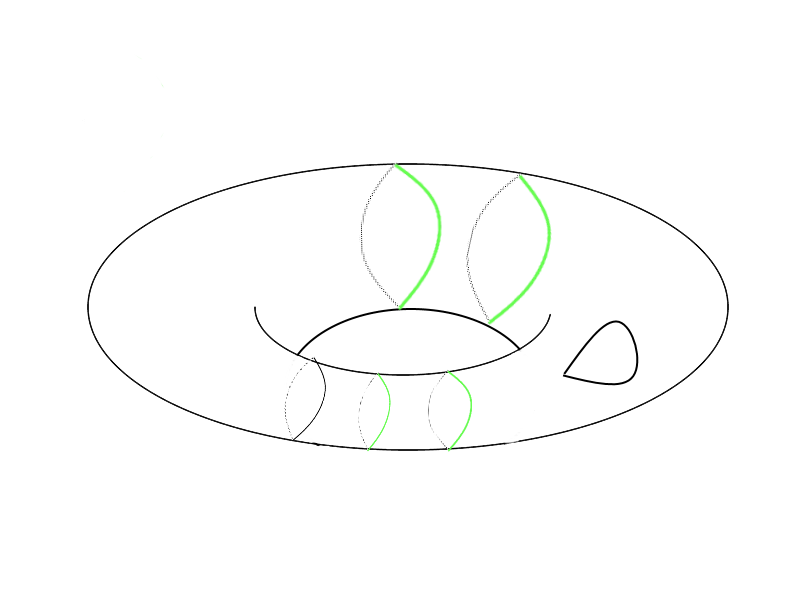
\includegraphics[width=\linewidth]{sample torus.png}
\end{subfigure}
\begin{subfigure}[b]{0.4\linewidth}
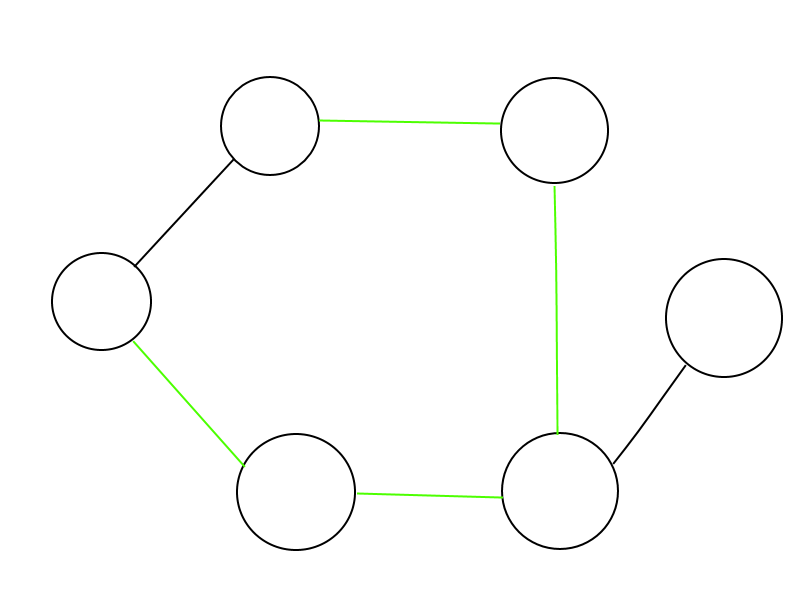
\includegraphics[width=\linewidth]{torus graph.png}
\end{subfigure}
\caption{The proof of Proposition \ref{existence of jump graphs} in case $M = \mathbf T^2$ and $u$ has two jump discontinuities, along each of the black loops. Note that we have to adjoin green leaves in order to ensure the simple connectedness condition, and that if we were to retract the green edges of the graph, then there would be a vertex of $I$ with a self-loop.}
\label{torus graphs}
\end{figure}
%%%%%%%%%%%%%%%%%%%%%%%%%%%%%%%%%%%%%%%%%%%%%%%%%

\subsection{Regularity of functions of least gradient}
In order to apply Proposition \ref{construction of minimal partitions}, it will be convenient to reduce to the cases that a given function $u$ of least gradient is either continuous, or the jump function of a lamination whose moduli space of leaves is discrete.
This will be possible if we prove Theorem \ref{Gorny regularity}, and thanks to Proposition \ref{construction of minimal partitions} this can be done.

\begin{lemma}
Let $u$ be a function of least gradient and $x \in M$. Then either the germ of $u$ at $x$ is continuous, or there exists a level set $N$ of $u$ such that $x \in N$ and the traces of $u$ along $N$ are constant and nonequal.
\end{lemma}
\begin{proof}
Reasoning identically to the proof of \cite[Proposition 3.9]{górny2017planar} (TODO Clarify this point) we see that $u$ jumps at $x$ iff
$$\inf\left\{t \in \RR: \lim_{r \to 0} \frac{|\{u \leq t\} \cap B(x, r)|}{|B(x, r)|} = 1\right\} \neq \sup\left\{t \in \RR: \lim_{r \to 0} \frac{|\{u \geq t\} \cap B(x, r)|}{|B(x, r)|} = 1\right\}.$$
The claim now follows from \cite[Theorem 4.1]{HakkarainenKorteLahtiShanmugalingam+2015}, which is true for functions of least gradient on metric measure spaces and in particular holds in our setting.
\end{proof}

\begin{proof}[Proof of Theorem \ref{Gorny regularity}]
Let $u$ be a function of least gradient on $M$ with jump set $J_u$.
Combining the above propositions TODO, there exists a unique (up to isomorphism) decomposition $u = u_j - u_c$ into sections $u_j, u_c: M \to E$, where $E$ is a flat affine line bundle with structure group $\RR$, such that $u_j$ is locally constant on $M \setminus \lambda$, $u_j$ has the same jumpset, with the same traces on each leaf, as $u$, and $u_c$ has no jump discontinuties.
Reasoning identically to \cite[pg11]{górny2017planar} we see that $u_j, u_c$ have locally least gradient.
Repeating the reasoning from the start of this proof and using the fact that $u_c$ has no jump discontinuities, it follows that $u_c$ is continuous.
\end{proof}

%%%%%%%%%%%%%%%%%%%%%%%%%%%%%%%%%%%%%%%

\subsection{Functions of least gradient induce minimal laminations}

\begin{definition}
A \dfn{minimal partition} is a closed set $\lambda$ which has been partitioned into (disjoint, embedded, without boundary) minimal hypersurfaces, called the \dfn{leaves} of $\lambda$.
\end{definition}

\begin{proposition}\label{construction of minimal partitions}
Let $u$ be a set of least gradient on $M$, $2 \leq d \leq 7$.
Then the connected components of the level sets $\partial \{u > y\}$ of $u$ define a minimal partition with support $\supp \dif u$, and each level set only has locally finitely many connected components, each of which is stable.
\end{proposition}
\begin{proof}
Let $\mathscr P$ be the set of all connected components of all level sets of $u$.
By \cite[Theorem 1]{BOMBIERI1969}, for every $y \in \RR$, $\{u > y\}$ has least perimeter.
The argument of \cite{BOMBIERI1969} only relies on the coarea formula and Miranda stability theorem, which we proved for manifolds in \S\ref{Prelims}, so it applies in our setting.
So by Theorem \ref{main thm}, $\{u > y\}$ is bounded by connected, embedded, stable minimal hypersurfaces; in particular, the elements of $\mathscr P$ are connected, embedded, stable minimal hypersurfaces.
Moreover, the decomposition of $\partial \{u > y\}$ into components is locally finite.
Indeed, by Corollary \ref{doubling dimension}, each connected component $N$ of $\partial \{u > y\}$ satisfies $|N \cap B| \gtrsim r^{d - 1}$, yet $\partial \{u > y\}$ has locally finite perimeter, thus $|\partial \{u > y\} \cap B| < \infty$.

We now show that any two distinct $N_1, N_2 \in \mathscr P$ are disjoint.
If $x \in N_1 \cap N_2$, then let $N_i$ be a component of $\partial \{u > y_i\}$.
Without loss of generality, $y_1 \leq y_2$, thus $\{u > y_2\} \subseteq \{u > y_1\}$, and hence $N_2 \subseteq \overline{\{u > y_1\}}$.
In particular $N_2$ lies on one side of $N_1$, so by the maximum principle, the germs of $N_1$ and $N_2$ at $x$ are identical.
So by unique continuation, $N_1 = N_2$.

The following statements are manifestly equivalent:
\begin{enumerate}
\item $x \notin \supp \dif u$.
\item The germ of $u$ at $x$ is constant.
\item If $u > y$ on one side of some hypersurface that passes through $x$, then $u > y$ near $x$.
\item $x \notin \partial \{u > y\}$ for any $y$.
\item $x \notin N$ for any leaf $N$ associated to $u$.
\end{enumerate}
It follows that $\supp \dif u$ is the support of the minimal partition whose set of leaves is $\mathscr P$.
\end{proof}

It is instructive to observe that the seemingly purely set-theoretic claims of the previous proposition require Theorem \ref{main lma}.
Indeed, in case $d = 8$, we could define for $x \in \RR^4$, $y \in \RR^3$, $z \in \RR$,
$$u(x, y, z) = \begin{cases}
-1, & z < 0 \\
0, & z > 0, |x|^2 < |y|^2 + z^2 \\
1, & z > 0, |x|^2 > |y|^2 + z^2
\end{cases}$$
and then the level sets of $u$ are the Simons cone $\{|x|^2 = |y|^2 + z^2\} \cap \{z \geq 0\}$ and the hyperplane $\{z = 0\}$, which intersect at $0$ and are minimal, thus $u$ has least gradient on $\RR^8$.

\begin{proof}[Proof of Theorem \ref{main thm}]
Let $u$ be a function of least gradient.
By Proposition \ref{construction of minimal partitions}, $\supp \dif u$ is the support of a minimal partition $\lambda$ whose leaves are the level sets of $u$, where each level set is the locally finite union of its components, and so by \cite[TODO]{BackusCML} $\lambda$ is a minimal lamination.

Let $(y_i, x_i): U_i \to Y_i \times N_i$, $i \in I$, be an atlas for $\lambda$.
Here $K_i \subseteq Y_i$ is the moduli space of leaves of $\lambda$ in $Y_i$.
Then, on the fibers $N_{y_i} := \{y_i\} \times N_i$, $u$ is constant.
Indeed, either $y_i \in K_i$ and so $N_{y_i}$ is contained in a level set of $u$, or $y_i \notin K_i$, so $N_{y_i}$ lies in a \dfn{plaque}, or component of $M \setminus \supp \lambda$, and hence $\dif u = 0$ in an open neighborhood of $N_{y_i}$.

In particular, we can define $u_i: Y_i \to \RR$ by setting $u_i(y_i) = u(y_i, x_i)$ for any $x_i \in N_i$.
Then $u_i$ satisfies the maximum principle: there do not exist $y_{i,1}$ and $y_{i,2}$ such that $u_i'(y_{i,1}) > 0$ and $u_i'(y_{i,2}) < 0$.
If there do, then we can replace $u$ with a competitor $\tilde u$ on $U_i$ by setting $\tilde u$ to be $u$ away from the region $\{y_{i,1} < y_i < y_{i,2}\}$ and to be constant on that region; then $\int_{U_i} \star |\dif \tilde u| < \int_{U_i} \star |\dif u|$ which contradicts that $u$ has least gradient.
So $u_i$ is either nondecreasing or nonincreasing on $Y_i$; if it is nonincreasing, we replace $y_i$ with $-y_i$.
With this convention, for any partition of unity $(\chi_i)$,
$$\normal^\sharp := \sum_{i \in I} \chi_i \frac{\grad y_i}{|\grad y_i|}$$
is a global section of the sphere bundle $SM$ which is normal to every leaf of $\lambda$. In particular, $\normal^\sharp$ defines an orientation $[\normal^\sharp]$ of $\lambda$.

We now define a transverse measure $\mu$ to $\lambda$.
First, by the G\'orny decomposition, there exist sections $u_j, u_c$ of locally least gradient such that $u_j$ is a jump section, $u_c$ is continuous, and $u = u_c + u_j$.
Then these define minimal laminations $\lambda_j, \lambda_c$.
Moreover, $\lambda_j$ is a \emph{discrete} lamination in that its moduli space of leaves $K_{j,i}$ in $U_i$ is a discrete set, so we can define an atomic measure $\mu_{j,i}(\{N\})$ to be the amount that $u_j$ jumps along $N$.
It is clear that the transition maps $\psi_{ik}$, $i,k \in I$, are measure-preserving.

As for the continuous part, we define a new (possibly non-Lipschitz) flow box coordinate $\tilde y_i$ by setting $\tilde y_i$ to equal $u_{c,i}$ on each leaf, and extend to the plaques by imposing that $\tilde y_i$ must be strictly increasing in $y_i$, and linear in $y_i$ on each plaque.
Then $y_i \mapsto \tilde y_i$ is a homeomorphism $Y_i \to \tilde Y_i$ for some $\tilde Y_i \subseteq \RR$, since $u_{c,i}$ is continuous and nondecreasing in $y_i$.
Here we are assuming that each flow box $U_i$ is contained in a trivialization of the affine line bundle of which $u_c$ is a section.
In particular, we may define for each Borel set $E \subset \tilde Y_i$,
$$\mu_{c,i}(E) := (\tilde y_i)_*(\star |\dif u|)(E) = \int_{(\tilde y_i)^*(E)} \star |\dif u|.$$
To see that $\psi_{ik}$ is measure-preserving we observe that $\psi_{ik}$ transforms $\tilde y_i$ to $\tilde y_k$, hence
$$\psi_{ik}^* \mu_{c,i} = \psi_{ik}^* (\tilde y_i)_* (\star |\dif u|) = (\tilde y_k)_* (\star |\dif u|) = \mu_{c,k}.$$

Summing up, $\mu_c, \mu_j$ are transverse measures and so their sum $\mu := \mu_c + \mu_j$ is also transverse.
By the disintegration theorem, for any $f \in L^1(\dif u)$,
$$\int_M f \star |\dif u| = \sum_{i \in I} \int_{K_i} \left[\int_{\{y_i\} \times N_i} \star_{y_i} \chi_i f \right] \dif \mu_i(y_i).$$
Here $\star_{y_i}$ is the Hodge star on $\{y_i\} \times N_i$ induced by $g$.
So for any $d-1$-form $\varphi$,
\begin{align*}
\int_M \dif u \wedge \varphi &= \int_M (\normal^\sharp, \varphi) \star |\dif u|
= \sum_{i \in I} \int_{K_i} \left[\int_{\{y_i\} \times N_i} \star_{y_i} \chi_i \star_{y_i} \varphi \dif \nu_{y_i}\right] \dif \mu_i(y_i) \\
&= \sum_{i \in I} \int_{K_i} \left[\int_{\{y_i\} \times N_i} \chi_i \varphi\right] \dif \mu_i(y_i)
\end{align*}
which implies that $\dif u$ is the Ruelle-Sullivan current of $(\lambda, [\normal^\sharp], \mu)$.

As for the converse, let $\lambda$ be a minimal lamination, and suppose that $\dif u$ is Ruelle-Sullivan for $\lambda$.
Then $\star |\dif u|$ is transverse to the leaves of $\lambda$, so $u$ is constant on each leaf.
Now let $U \Subset M$ and let $v \in BV_\cpt(U)$, thus $V = U \setminus \supp v$ is the intersection of an open neighborhood of $\partial U$ with $U$.
If $v$ is not identically zero, then there is a positive measure set $Y \subseteq \RR$ such that for $y \in Y$, $\partial \{u > y\} \neq \partial^* \{u + v > y\}$.
But
$$V \cap \partial \{u > y\} = V \cap \partial^* \{u + v > y\}$$
so $1_{\{u > y\}}$ and $1_{\{u + v > y\}}$ are equalized by the trace map $BV_\loc(U) \to L^1_\loc(\partial U)$.
Now $\{u > y\}$ has least perimeter in $U$, so if $|U \cap \partial \{u > y\}| = |U \cap \partial^* \{u + v > y\}|$ then $\{u + v > y\}$ has least perimeter in $U$.
Each component of $\partial \{u > y\}$ and $\partial \{u + v > y\}$ is a minimal hypersurface in $U$ with the same trace, so by unique continuation,
$$\partial \{u > y\} = \partial \{u + v > y\}.$$
But this contradicts the assumption that $y \in Y$. So for each $y \in Y$,
$$|U \cap \partial \{u > y\}| < |U \cap \partial^* \{u + v > y\}|.$$
Integrating both sides in $y$ using the coarea formula, we conclude that
\begin{align*}
\int_U \star |\dif u + \dif v| - \star |\dif u| &= \int_{-\infty}^\infty |U \cap \partial^* \{u + v > y\}| - |U \cap \partial \{u > y\}| \dif y \\
&= \int_Y |U \cap \partial^* \{u + v > y\}| - |U \cap \partial \{u > y\}| \dif y > 0,
\end{align*}
and since $v$ was an arbitrary perturbation, $u$ must have least gradient.
\end{proof}

